\section{Results}
\label{sec:results}

We report three results in sequence. First, a first-stage check: the
patient-flow exposure rule captures populations with realized utilization
ties to the closing hospital, evidenced by a sharp fall in travel burden
(\ref{sec:results-firststage}). Second, the headline: among those
exposed populations, the data do not show a large acute mortality
increase (\ref{sec:results-mortality}). Third, a result we decline to
read causally: preventable hospitalizations rise after closure, but they
were already rising before it (\ref{sec:results-icsap}). The full
robustness battery is in Section~\ref{sec:robustness}.

% =====================================================================
% §5.1 — First stage
% =====================================================================
\subsection{First stage: the flow rule captures realized dependence}
\label{sec:results-firststage}

Before asking what happened to the exposed populations, we verify that
the flow exposure rule identifies municipalities with realized admission
links to the closing hospital rather than ones merely near it. The test is
mechanical and sharp: if exposed patients had been traveling far for
care at the closing facility, then closure should change the distance
they travel for inpatient care, because the long trips the facility
generated cease or are replaced by other utilization.

Figure~\ref{fig:firststage-travel} reports the staggered event study for
travel burden. The pre-period coefficients are flat---the joint
Wald-style test does not reject parallel trends ($p = \valTravPpre$)---and travel
burden falls by $\valTravAbs$~km in the post-period (95\% CI $[\valTravLo, \valTravHi]$;
Table~\ref{tab:mortality-null}, first row). A distance-based exposure
rule applied to the same closures recovers only about half this
magnitude, because it dilutes the flow-dependent municipalities
with geographically near ones whose residents never used the closing
hospital. The fall confirms that flow-exposed municipalities were
sending patients on long trips to the facility that closed. It shows
where the closing hospital mattered in realized utilization; it does not
by itself distinguish lost care from substitution to nearer providers.

\begin{figure}[h!]
    \centering
    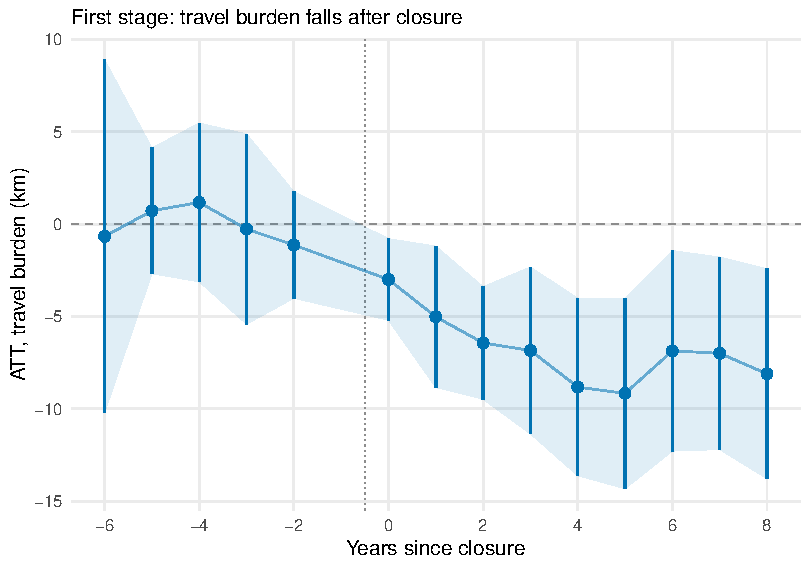
\includegraphics[width=0.6\textwidth]{../04_figures/fig_firststage_travel.pdf}
    \caption{First stage. Staggered Sun-Abraham event study for travel
    burden (km) on the $\valNclosuresPnash$ PNASH-anchored psychiatric closures and
    their $\valNtrPnash$ flow-exposed municipalities. Pre-period coefficients
    test parallel trends; the dotted line marks the pre/post boundary.
    Bars are $95\%$ cluster-robust confidence intervals. Travel burden
    falls after closure, showing that exposed municipalities had been
    sending patients on long trips to the closing hospital.}
    \label{fig:firststage-travel}
\end{figure}

% =====================================================================
% §5.2 — The mortality null (headline)
% =====================================================================
\subsection{Mortality: ruling out large acute increases}
\label{sec:results-mortality}

We now ask the policy question directly: did closing the psychiatric
hospitals raise mortality among the populations that depended on them?
We estimate effects on two outcomes recorded at the municipality of
residence---suicide (ICD-10 X$60$--X$84$) and a broader self-harm
measure that adds deaths of undetermined intent (Y$10$--Y$34$)---both
expressed per $100{,}000$ inhabitants. We report population-weighted
estimates as primary, because the policy-relevant quantity is the effect
on the average exposed \emph{person}, not the average exposed
municipality; the municipality-weighted estimate is the unweighted
complement.

Figure~\ref{fig:es-mortality} reports the event-study
trajectories and Table~\ref{tab:mortality-null} the summary estimates.
Population-weighted suicide mortality changes by $\valSuicWAtt$ per $100{,}000$
after closure (95\% CI $[\valSuicWLo, \valSuicWHi]$), with pre-period coefficients
that are flat and a parallel-trends test that does not reject
($p = \valSuicWPpre$). Self-harm mortality is likewise indistinguishable from
zero ($\valSelfWAtt$, 95\% CI $[\valSelfWLo, \valSelfWHi]$, $p_{\text{pre}} = \valSelfWPpre$). The
municipality-weighted estimates are, if anything, negative and remain
statistically null. Across every specification the post-period
trajectory hovers around zero with no upward drift large enough to be
visible in these data.

What this null does and does not establish deserves precision. The
upper bound of the suicide confidence interval is $\valSuicWHi$ per
$100{,}000$, roughly one-quarter of the treated-group baseline. The
estimate therefore \emph{rules out} large acute mortality increases---a
one-quarter rise in suicide among the exposed would lie outside the
interval---but it does \emph{not} establish a precise zero: effects
smaller than that bound the data cannot resolve at
$N = \valNclosuresPnash$ closures (formal
minimum detectable effects are in Appendix~\ref{app:power}). The policy reading is
correspondingly bounded. The data do not show the large acute mortality
increase critics feared; they cannot speak to subtle harms or
non-mortality welfare margins.

\begin{table}[h!]\centering
\caption{Mortality effects of psychiatric hospital closures. Staggered Sun-Abraham ATT on patient-flow--exposed municipalities, pre-periods observed back to 2010. Population-weighted rows give the effect on the average exposed person (the policy-relevant quantity); municipality-weighted rows are the unweighted complement. ``Upper bound'' is the 95\% CI upper limit as a share of the pre-treatment treated-group baseline. Cluster-robust SE at the municipality level.}
\label{tab:mortality-null}\small
\resizebox{\textwidth}{!}{%
\begin{tabular}{llccccc}
\toprule
 & Weighting & ATT & 95\% CI & Upper bound & Pre-trend $p$ & $N_{\text{tr}}$ \\
\midrule
\multicolumn{7}{l}{\textit{First stage --- realized utilization links}}\\
Travel burden (km) & --- & $-7.09$ & $[-11.07,\,-3.10]$ & $-6\%$ & 0.96 & 104 \\
\addlinespace
\multicolumn{7}{l}{\textit{Mortality among flow-exposed municipalities}}\\
Suicide (per 100k) & Population & $+0.28$ & $[-0.72,\,+1.29]$ & $+26\%$ & 0.26 & 104 \\
 & Municipality & $-2.10$ & $[-5.01,\,+0.82]$ & $+13\%$ & 0.15 & 104 \\
Self-harm (per 100k) & Population & $+0.61$ & $[-0.90,\,+2.12]$ & $+28\%$ & 0.53 & 104 \\
 & Municipality & $-0.79$ & $[-4.41,\,+2.82]$ & $+31\%$ & 0.19 & 104 \\
\addlinespace
\multicolumn{7}{l}{\textit{Robustness --- suicide, population-weighted, alternative closure samples}}\\
Specialized exogenous ($n{=}41$) & Population & $+0.36$ & $[-0.65,\,+1.37]$ & $+25\%$ & 0.10 & 105 \\
All psychiatric ($n{=}60$) & Population & $+0.34$ & $[-0.62,\,+1.31]$ & $+25\%$ & 0.23 & 112 \\
\bottomrule
\multicolumn{7}{l}{\footnotesize Primary sample: 48 PNASH-anchored psychiatric closures, 104 exposed municipalities, 2010--2024.}\\
\end{tabular}
}%
\end{table}


\begin{figure}[h!]
    \centering
    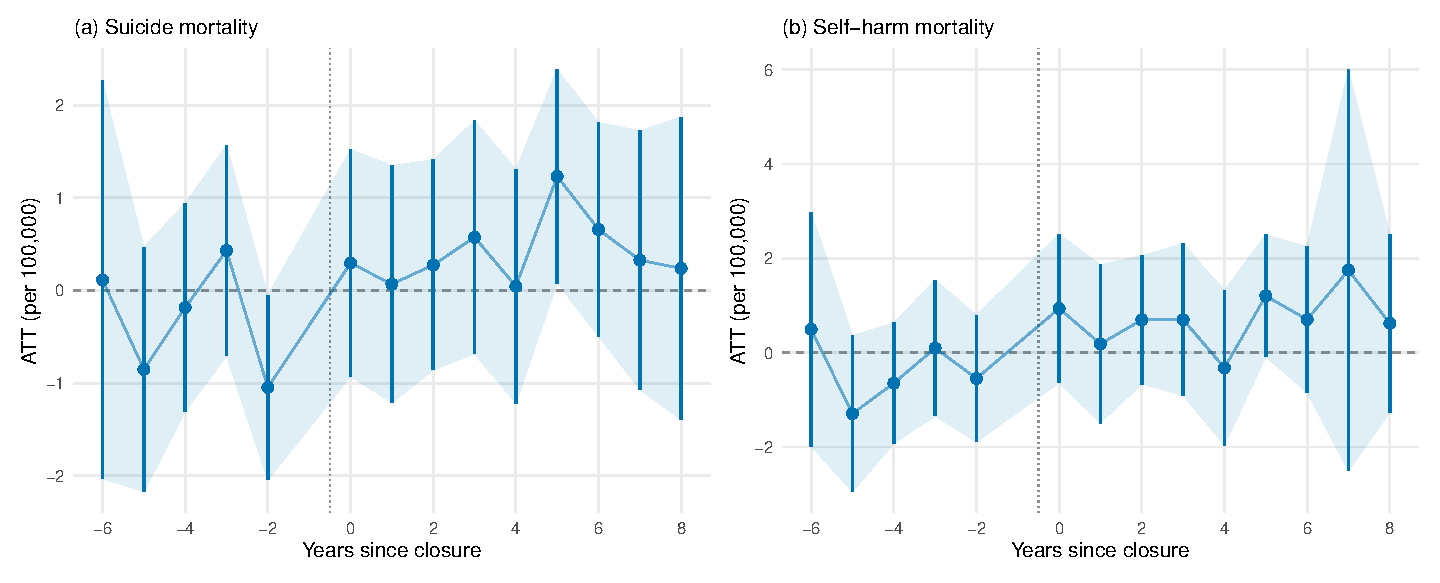
\includegraphics[width=0.95\textwidth]{../04_figures/fig_es_mortality.pdf}
    \caption{Mortality event studies. Population-weighted staggered
    Sun-Abraham event studies for (a) suicide and (b) self-harm
    mortality per $100{,}000$, on the $\valNclosuresPnash$ PNASH-anchored psychiatric
    closures. Pre-periods are observed back to $2010$. Both trajectories
    are flat before closure and remain indistinguishable from zero
    after. Bars are $95\%$ cluster-robust confidence intervals.}
    \label{fig:es-mortality}
\end{figure}

\paragraph{Population versus municipality weighting.} The point
estimates differ in sign between the two weightings---population-weighted
slightly positive, municipality-weighted slightly negative---which
reflects that the effect, to the extent there is one, differs between
small and large exposed municipalities, not that the result is fragile.
Both weightings deliver imprecise estimates around zero with confidence
intervals that exclude large increases; the disagreement is in the
second decimal, not in the conclusion. We lead with the
population-weighted estimate because it answers the policy question
(harm to people, not to places), and report the municipality-weighted
estimate so that the reader can see the null is not an artifact of
down-weighting small areas.

% =====================================================================
% §5.3 — The declined non-result (ICSAP)
% =====================================================================
\subsection{A result we decline to read causally}
\label{sec:results-icsap}

A credible null requires being as honest about the outcomes we cannot
identify as about the one we can. Preventable hospitalizations
(ICSAP)---the canonical Brazilian access-to-care marker
\citep{macinkoHarris2015, rochaSoares2010}---do rise after closure in
the exposed municipalities, by $\valIcsapAtt$ per $1{,}000$ in the post-period.
Read naively, this could look like the access deterioration one would expect
if closures pushed unmet need into preventable hospitalizations. It is
not identified.

Figure~\ref{fig:es-icsap-pretrend} shows why. With the pre-periods
observed back to $2010$, the pre-treatment coefficients are large and
significantly positive---$\valIcsapPreThree$, $\valIcsapPreFour$, and $\valIcsapPreFive$ per $1{,}000$ at
three, four, and five years before closure---and the parallel-trends
test rejects decisively ($p < 0.001$); a Rambachan-Roth sensitivity
confirms that no bounded extrapolation of the pre-trend rescues the
estimate (Appendix~\ref{app:rr}). ICSAP was already climbing in the
exposed municipalities well before any hospital closed; the post-closure
level is the continuation of a pre-existing trend, not a treatment
effect. We had earlier mistaken this for a clean result when the
pre-2015 data were missing and the pre-period appeared empty; with the
population denominators backfilled to $2010$, the trend is visible and
the apparent effect dissolves.

We therefore report the ICSAP trajectory in full and treat it as a
non-identified outcome. We do not bound it, do not interpret it
causally, and do not let it carry weight in the paper's conclusions.
The identified result is the mortality null; the ICSAP series is
informative only as a description of where the exposed municipalities
were already heading.

\begin{figure}[h!]
    \centering
    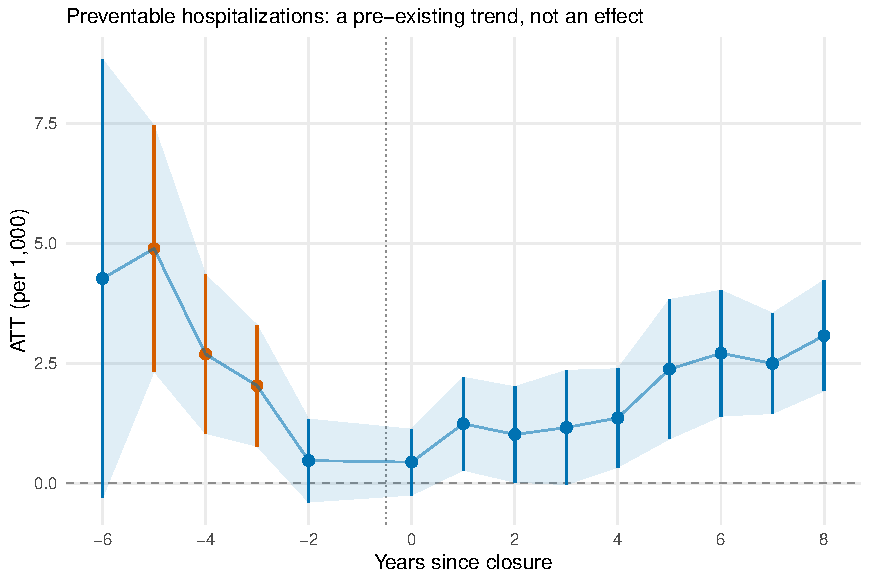
\includegraphics[width=0.62\textwidth]{../04_figures/fig_es_icsap_pretrend.pdf}
    \caption{A pre-existing trend, not an effect. Staggered event study
    for preventable hospitalizations (ICSAP) per $1{,}000$, pre-periods
    observed back to $2010$. Pre-treatment coefficients (highlighted)
    are large and significantly positive: ICSAP was already rising in
    the exposed municipalities before closure. The parallel-trends test
    rejects ($p < 0.001$), so we decline to read the post-closure level
    as a treatment effect.}
    \label{fig:es-icsap-pretrend}
\end{figure}
